\section{Practice Problem 6.5}
\begin{figure}[h!]
    \centering
    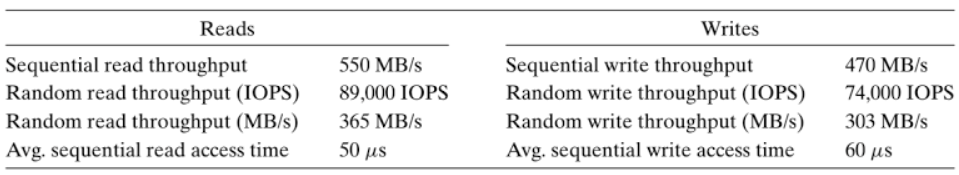
\includegraphics[width=\textwidth]{figures/ssd_props.png}
    \caption{Performance characteristics of a commercial solid state disk. 
    Source: Intel SSD 730 product specifictations. IOPS is I/O per seconds.
    throughput numbers are based on reads and writes of 4 KB blocks. (Intel SSD 730 product specifictations. Intel Cooperation)}
    \label{fig:ssd_specs}
\end{figure}
As we have seen, a potential drawback of SSDs is that the underlying flash memory can wear out.
For example, for the SSD in \cref{fig:ssd_specs}, Intel guarantees about 128 petabytes ($128\cdot 10^{15}$) of writes before the drive wears out.
Given this assumption, estimate the lifetime (in years) of this SSD for the following workloads:
\begin{enumerate}
    \item \textit{Wors case for sequential writes:} The SSD is written to continuously at a rate of 470 MB/s (The average sequential write throughput of the device).
    \item \textit{Worst case for random writes:} The SSD is written to continuously at a rate of 303 MB/s (the average random write throughput of the device)
    \item \textit{Average case:} The SSD is written to at a rate of 20 GB/day (the average daily write rate assumed by some computer manufacturers in their mobile computer workload simulations)
\end{enumerate}
\subsection{Udregninger til 6.5}
Det er givet at $1PB=10^9MB$. Samtidig vides det at der er 86400 sekunder på en dag.
\begin{enumerate}
    \item {
        Med denne information kan følgende formel bruges til at udregne levetiden for en SSD ved worst case load:
        \begin{equation}
            \left(10^9\cdot 128\right)\cdot\left(\frac{1}{470}\right)\cdot\left(\frac{1}{\left(86400\cdot 365\right)}\right) = \frac{800000}{92637} \approx 8.6359
        \end{equation}
    }
    \item {
        Samme formel kan bruges til at udregne worst case for random writes
        \begin{equation}
            \left(10^9\cdot 128\right)\cdot\left(\frac{1}{303}\right)\cdot\left(\frac{1}{\left(86400\cdot 365\right)}\right) = \frac{8000000}{597213} \approx 13.396
        \end{equation}
    }
    \item {
        Formlen kan også bruges til at udregne vores average case. 
        Dog skal sekunder ikke bruges i dette tilfælde, da der arbejdes med en tidsfaktor af dage.
        \begin{equation}
            \left(10^9\cdot 128\right)\cdot\left(\frac{1}{20000}\right)\cdot\left(\frac{1}{365}\right) = \frac{1280000}{73} \approx 17534.24658
        \end{equation}
    }
\end{enumerate}
Udregningerne er i år.